\documentclass[pdflatex,sn-mathphys-num]{sn-jnl}% Math and Physical Sciences Numbered Reference Style

%%\documentclass[pdflatex,sn-mathphys-ay]{sn-jnl}% Math and Physical Sciences Author Year Reference Style
%%\documentclass[pdflatex,sn-aps]{sn-jnl}% American Physical Society (APS) Reference Style
%%\documentclass[pdflatex,sn-vancouver-num]{sn-jnl}% Vancouver Numbered Reference Style
%%\documentclass[pdflatex,sn-vancouver-ay]{sn-jnl}% Vancouver Author Year Reference Style
%%\documentclass[pdflatex,sn-apa]{sn-jnl}% APA Reference Style
%%\documentclass[pdflatex,sn-chicago]{sn-jnl}% Chicago-based Humanities Reference Style

%%%% Standard Packages
%%<additional latex packages if required can be included here>
\usepackage{graphicx}
\usepackage{caption}
%\usepackage{subfigure}
\usepackage{subcaption}
\usepackage{booktabs}
\usepackage{longtable}

\usepackage{dsfont}
\usepackage{graphicx}%
\usepackage{multirow}%
\usepackage{amsmath,amssymb,amsfonts}%
\usepackage{amsthm}%
\usepackage{mathrsfs}%
\usepackage[title]{appendix}%
\usepackage{xcolor}%
\usepackage{textcomp}%
\usepackage{manyfoot}%
\usepackage{booktabs}%
\usepackage{algorithm}%
\usepackage{algorithmicx}%
\usepackage{algpseudocode}%
\usepackage{listings}%
%\usepackage{tcolorbox}
\usepackage[most]{tcolorbox}
\usepackage{adjustbox}
\usepackage{array}
\usepackage[utf8]{inputenc}
\usepackage{threeparttable}

\usepackage{soul} % \hl{}
\sethlcolor{green!18} % soft highlight; adjust if desired

% Timeline drawing
\usepackage{tikz}
\usetikzlibrary{arrows.meta,positioning}

\usepackage{fancyvrb}      % for Verbatim with inline commands
\usepackage[T1]{fontenc}   % ensures bold typewriter is available
\usepackage{lmodern}       % modern fonts (bold tt)
\usepackage{amsmath}
\usepackage{cleveref}

% Custom margins: left 2in, right 0.75in, top and bottom 1in (consistent on all pages)
\geometry{left=5cm, right=1.5cm, top=1.5cm, bottom=1.5cm, asymmetric}

% Override title page font definitions to use left alignment
\makeatletter

% Redefine fonts to use raggedright instead of titraggedcenter
\def\Titlefont{\reset@font\fontsize{17bp}{22.5bp}\selectfont\raggedright}%
\def\SubTitlefont{\reset@font\fontsize{14bp}{16.5bp}\selectfont\raggedright}%
\def\Authorfont{\reset@font\fontsize{12bp}{14.5bp}\selectfont\boldmath\raggedright}%
\def\addressfont{\reset@font\fontsize{11bp}{13.5bp}\selectfont\raggedright}%
\def\abstractheadfont{\reset@font\fontsize{9bp}{11bp}\bfseries\selectfont\raggedright}%
\def\abstractfont{\reset@font\fontsize{9bp}{11bp}\selectfont\raggedright}%

\newcommand{\jeremy}[1]{\textcolor{red}{#1}}
% Redefine main body text sizes (slightly smaller)
\renewcommand\normalsize{%
   \@setfontsize\normalsize{9.5bp}{11.4bp}%
   \abovedisplayskip 12\p@ \@plus2\p@ \@minus1\p@
   \abovedisplayshortskip \z@ \@plus3\p@%
   \belowdisplayshortskip 3\p@ \@plus3\p@ \@minus3\p@%
   \belowdisplayskip \abovedisplayskip%
   \let\@listi\@listI}%

\renewcommand\small{%
   \@setfontsize\small{8.5bp}{10.2bp}%
   \abovedisplayskip 5\p@ \@plus3\p@ \@minus4\p@
   \abovedisplayshortskip \z@ \@plus2\p@
   \belowdisplayshortskip 3\p@ \@plus2\p@ \@minus2\p@
   \def\@listi{\leftmargin\leftmargini
               \topsep 4\p@ \@plus2\p@ \@minus2\p@
               \parsep 2\p@ \@plus\p@ \@minus\p@
               \itemsep \parsep}%
   \belowdisplayskip \abovedisplayskip}%

\renewcommand\footnotesize{%
   \@setfontsize\footnotesize{7bp}{8bp}%
   \abovedisplayskip 5\p@ \@plus2\p@ \@minus4\p@
   \abovedisplayshortskip \z@ \@plus\p@
   \belowdisplayshortskip 3\p@ \@plus\p@ \@minus2\p@
   \def\@listi{\leftmargin\leftmargini
               \topsep 3\p@ \@plus\p@ \@minus\p@
               \parsep 2\p@ \@plus\p@ \@minus\p@
               \itemsep \parsep}%
   \belowdisplayskip \abovedisplayskip}%

% Redefine section header fonts (smaller)
\def\sectionfont{\reset@font\fontfamily{\rmdefault}\fontsize{12bp}{14bp}\bfseries\selectfont\raggedright\boldmath}%
\def\subsectionfont{\reset@font\fontfamily{\rmdefault}\fontsize{10.5bp}{12.5bp}\bfseries\selectfont\raggedright\boldmath}%
\def\subsubsectionfont{\reset@font\fontsize{9.5bp}{11.5bp}\bfseries\selectfont\raggedright\boldmath}%
\def\paragraphfont{\reset@font\fontsize{9bp}{11bp}\bfseries\itshape\selectfont\raggedright}%

% Reduce top spacing on title page
\renewcommand{\@maketitle}{\newpage\null%
    \if@remarkboxon\vbox to 0pt{\vspace*{-78pt}\hspace*{-18pt}\FMremark}\else\vskip-10pt\fi% Changed from \vskip21pt to \vskip-10pt
    \hsize\textwidth\parindent0pt%
    {\hbox to \textwidth{{\Artcatfont\ArtType\hfill}\par}}%
    \ifx\@title\empty\else%
        \removelastskip\vskip20pt\nointerlineskip%
        {\Titlefont\@title\par}%
    \fi%
    \ifx\@subtitle\empty\else%
        \vskip9pt%
        {{\SubTitlefont\@subtitle\par}}%
    \fi%
    \ifnum\aucount>0
        \global\punctcount\aucount%
        \vskip20pt%
        \artauthors\par%
        {\vskip7pt\addressfont\auaddress\par%
	 \removelastskip\vskip24pt%
	\ifnum\emailcnt>0\relax%
           \ifx\corrauthemail\@empty\else{\ifnum\aucount>1*\fi}%
	   Corresponding author(s). E-mail(s): \corrauthemail\par\fi%
	   \ifx\authemail\@empty\else Contributing authors:\ \authemail\fi%
        \fi%
        \ifequalcont{\par$^{\dagger}$\@equalconttext\par}\fi%
	 \removelastskip\vskip24pt%
        \ifpresentaddress{\par\@presentaddresstext\par}\fi%
	}%
     \fi%
     {\printabstract\par}%
     {\printkeywords\par}%
     \ifx\@pacs\empty\else%
       \loop\ifnum\PacsCount>0%
          \csname\romannumeral\PacsTmpCnt StorePacsTxt\endcsname\par%
          \StepDownCounter{\PacsCount}%
          \StepUpCounter{\PacsTmpCnt}%
       \repeat%
    \fi%
    \removelastskip\vskip36pt\vskip0pt}%

\makeatother

%%%%

%%%%%=============================================================================%%%%
%%%%  Remarks: This template is provided to aid authors with the preparation
%%%%  of original research articles intended for submission to journals published 
%%%%  by Springer Nature. The guidance has been prepared in partnership with 
%%%%  production teams to conform to Springer Nature technical requirements. 
%%%%  Editorial and presentation requirements differ among journal portfolios and 
%%%%  research disciplines. You may find sections in this template are irrelevant 
%%%%  to your work and are empowered to omit any such section if allowed by the 
%%%%  journal you intend to submit to. The submission guidelines and policies 
%%%%  of the journal take precedence. A detailed User Manual is available in the 
%%%%  template package for technical guidance.
%%%%%=============================================================================%%%%

%% as per the requirement new theorem styles can be included as shown below
\theoremstyle{thmstyleone}%
\newtheorem{theorem}{Theorem}%  meant for continuous numbers
%%\newtheorem{theorem}{Theorem}[section]% meant for sectionwise numbers
%% optional argument [theorem] produces theorem numbering sequence instead of independent numbers for Proposition
\newtheorem{proposition}[theorem]{Proposition}% 
%%\newtheorem{proposition}{Proposition}% to get separate numbers for theorem and proposition etc.

\theoremstyle{thmstyletwo}%
\newtheorem{example}{Example}%
\newtheorem{remark}{Remark}%

\theoremstyle{thmstylethree}%
\newtheorem{definition}{Definition}%

\raggedbottom
%%\unnumbered% uncomment this for unnumbered level heads


% %-------------------------------------------------
% % Supplementary Material Formatting for sn-jnl
% %-------------------------------------------------

% \makeatletter

% % Completely suppress the default "Appendix A" title
% \renewcommand\appendix{\par
%   \setcounter{section}{0}%
%   \setcounter{subsection}{0}%
%   \setcounter{subsubsection}{0}%
%   \gdef\thesection{S\arabic{section}}%
%   \gdef\thesubsection{S\arabic{section}.\arabic{subsection}}%
%   \gdef\thesubsubsection{S\arabic{section}.\arabic{subsection}.\arabic{subsubsection}}%
%   \renewcommand{\thefigure}{S\arabic{figure}}%
%   \renewcommand{\thetable}{S\arabic{table}}%
%   \renewcommand{\theequation}{S\arabic{equation}}%
% }

% % Remove the automatic "Appendix" heading inserted by the class
% % \renewcommand\@makechapterhead[1]{}
% % \renewcommand\@makeschapterhead[1]{}

% \makeatother

%%%%%%%%%%%%%%%%%%%%%%%%%%%%%%%%%%%%%%%%%%%%%%%%%%%
%%%%%%%%%%%%%%%%%%%%%%%%%%%%%%%%%%%%%%%%%%%%%%%%%%%

\begin{document}

\title[Article Title]{Temporally annotated textual time series from PubMed Open Access clinical case reports}

%%=============================================================%%
%% GivenName	-> \fnm{Joergen W.}
%% Particle	-> \spfx{van der} -> surname prefix
%% FamilyName	-> \sur{Ploeg}
%% Suffix	-> \sfx{IV}
%% \author*[1,2]{\fnm{Joergen W.} \spfx{van der} \sur{Ploeg} 
%%  \sfx{IV}}\email{iauthor@gmail.com}
%%=============================================================%%

\author[1,2]{\fnm{Shahriar} \sur{Noroozizadeh}}\email{snoroozi@cs.cmu.edu}
\equalcont{These authors contributed equally to this work.}

\author[3]{\fnm{Sayantan} \sur{Kumar}}\email{sayantan.kumar@nih.gov}
\equalcont{These authors contributed equally to this work.}

\author[2,1]{\fnm{George H.} \sur{Chen}}\email{georgechen@cmu.edu}

\author*[3]{\fnm{Jeremy C.} \sur{Weiss}}\email{jeremy.weiss@nih.gov}

\affil[1]{\orgdiv{Machine Learning Department, School of Computer Science}, \orgname{Carnegie Mellon University}, \city{Pittsburgh}, \state{Pennsylvania}, \country{USA}}

\affil[2]{\orgdiv{Heinz College of Information Systems and Public Policy}, \orgname{Carnegie Mellon University}, \city{Pittsburgh}, \state{Pennsylvania}, \country{USA}}

\affil[3]{\orgdiv{National Library of Medicine}, \orgname{National Institutes of Health}, \orgaddress{%\street{Street},
\city{Bethesda}, \state{Maryland}, \country{USA}}}

%%==================================%%
%% Sample for unstructured abstract %%
%%==================================%%

\abstract{
Clinical narratives encode temporal dynamics essential for modeling patient trajectories, yet large-scale temporally annotated resources are scarce. We introduce PMOA–TTS, a corpus of 124,699 single-patient PubMed Open Access case reports converted into structured textual timelines of (event, time) pairs using a scalable large-language-model pipeline (\texttt{Llama 3.3 70B} and \texttt{DeepSeek-R1}). The corpus comprises over 5.6 million timestamped events, alongside extracted demographics and diagnoses. Technical validation uses a clinician-curated gold set and three measures: semantic event matching, temporal concordance (c-index), and alignment error summarized with Area Under the Log-Time CDF (AULTC). We benchmark alternative prompting and model choices and provide documentation to support reproduction. PMOA–TTS enables research on timeline extraction, temporal reasoning, survival modeling and event forecasting from narrative text, and offers broad diagnostic and demographic coverage. Data and code are openly available in public repositories.
}

%\keywords{keyword1, Keyword2, Keyword3, Keyword4}
\keywords{clinical natural language processing, temporal information extraction, textual time series, large language models, PubMed Open Access case reports}

\maketitle

% Background & Summary
% Methods
% Data Records
% Data Overview (optional)
% Technical Validation
% Usage Notes (optional)
% Data Availability
% Code Availability
% References
% Author Contributions
% Competing Interests
% Acknowledgements (optional)
% Funding
% Ethics statement* 

%%%%%%%%%%%%%%%%%%%%%%%%%%%%%%%%%%%%%%%%%%%%%%
%%%%%%%%%%%%%% Introduction %%%%%%%%%%%%%%%%%
%%%%%%%%%%%%%%%%%%%%%%%%%%%%%%%%%%%%%%%%%%%%%
\section{Introduction}
\label{sec:introduction}

Understanding when clinical events occur is fundamental to modeling patient trajectories, enabling tasks such as process mining, outcome forecasting, and causal inference in medicine \citep{jensen2012mining, noren2010temporal}.
However, most clinical narratives lack explicit temporal structure. While electronic health record (EHR) datasets like MIMIC-III and MIMIC-IV include timestamped structured data and clinical notes \citep{johnson2016mimic, johnson2023mimic}, they capture only a subset of events (e.g., vital signs, lab results) and still require sophisticated natural language processing to extract temporal information from unstructured text \citep{viani2021temporal, cheng2023typed}.

In contrast, published case reports often provide rich narrative descriptions of patient timelines, but the timing of events is typically expressed in relative terms within the free text (e.g., “on day 3 of hospitalization”).
Efforts in temporal reasoning on clinical text have been hampered by the scarcity of large-scale annotated corpora.
Earlier initiatives, such as the 2012 i2b2 challenge and Clinical TempEval, focused on temporal relation extraction from clinical notes \citep{sun2013evaluating, bethard2016semeval, galvan2018investigating} but were constrained by small datasets (e.g., 310 documents) from single institutions, limiting model performance and generalizability.
Systems that rely on metadata timestamps (e.g., admission or discharge dates) fail to capture the fine-grained sequence of clinical events described in text, which is essential for nuanced understanding and prediction.
There remains a pressing need for large-scale, temporally annotated corpora to support the development and evaluation of models for clinical temporal reasoning.

Building on our pilot pipeline on 20 case reports \citep{wang2025large}, we introduce the PubMed Open Access Textual Time Series (PMOA–TTS) corpus—a large-scale dataset of 124,699 openly available clinical case reports, each annotated with a structured timeline of events.
Leveraging large language models (LLMs)—specifically \texttt{Llama 3.3 70B} \citep{grattafiori2024llama} and \texttt{DeepSeek-R1} \citep{guo2025deepseek}—we transform each case report into a sequence of \mbox{(clinical event, time)} tuples that capture key clinical events and their relative timing within the patient narrative (Figure \ref{fig:annotation_ex}).
To our knowledge, PMOA–TTS constitutes the largest publicly available collection of clinical narratives with explicit temporal event structure.
We demonstrate that these temporal annotations enable novel forms of analysis and significantly enhance downstream modeling of patient outcomes.

Building PMOA--TTS requires addressing three challenges at scale: reliably identifying single-patient case reports, extracting timeline events with high fidelity from ambiguous free-text time expressions, and rigorously evaluating the resulting annotations. We meet these needs with an LLM-based pipeline that selects relevant narratives beyond naive metadata filters, resolves relative time language into fine-grained event--time tuples, and enriches each case with structured demographics and diagnoses. To illustrate practical value, we also formulate a downstream survival analysis task that operates directly on the extracted textual time series.

\input{Scientific_data/Figures_Tables/TTS_example_figure}

In summary, we (i) introduce the PMOA Textual Time Series (PMOA--TTS) corpus of 124{,}699 single-patient case reports from PubMed Open Access, each annotated with structured clinical timelines extracted using large language models; (ii) develop a scalable pipeline for automatic case identification and prompt-driven extraction of timelines, demographics, and diagnoses, together with a manual evaluation framework; (iii) define and apply complementary validation measures for timeline accuracy, including temporal order concordance (c-index) and the Area Under the Log-Time CDF (AULTC); (iv) characterize corpus properties (demographics, frequent diagnoses, and co-occurrence structure) to document clinical and demographic breadth; and (v) illustrate one reuse pathway by framing survival prediction directly over textual time series.

PMOA–TTS offers several potential positive contributions to the biomedical NLP and clinical AI communities. By releasing the largest openly available dataset of temporally structured clinical narratives, this work democratizes access to timeline-based clinical text—an area typically limited to proprietary EHR datasets. The corpus spans a wide range of diagnoses and demographics, supporting research on temporal patterns in diverse and sometimes underrepresented conditions. Additionally, by making the extraction pipeline, prompting strategies, and evaluation framework publicly available, the project promotes transparency and reproducibility in LLM-based clinical information extraction. These contributions collectively advance the development of models for timeline reconstruction, temporal reasoning, and longitudinal prediction, while lowering the barrier
to entry for researchers working in resource-limited settings.


%%%%%%%%%%%%%%%%%%%%%%%%%%%%%%%%%%%%%%%%%%%%%%%%%%%
%%%%%%%%%%%%%% Methods %%%%%%%%%%%%%%%%%%%%%%%%%%%
%%%%%%%%%%%%%%%%%%%%%%%%%%%%%%%%%%%%%%%%%%%%%%%%%%

\section{Methods}
\label{sec:methods}

Our pipeline comprises the following key components: dataset extraction, textual time series annotation, and comprehensive evaluation of the annotations (Figure~\ref{fig:flowchart}).

\begin{figure}[!htbp] % 'r' for right, 'l' for left
    \centering
    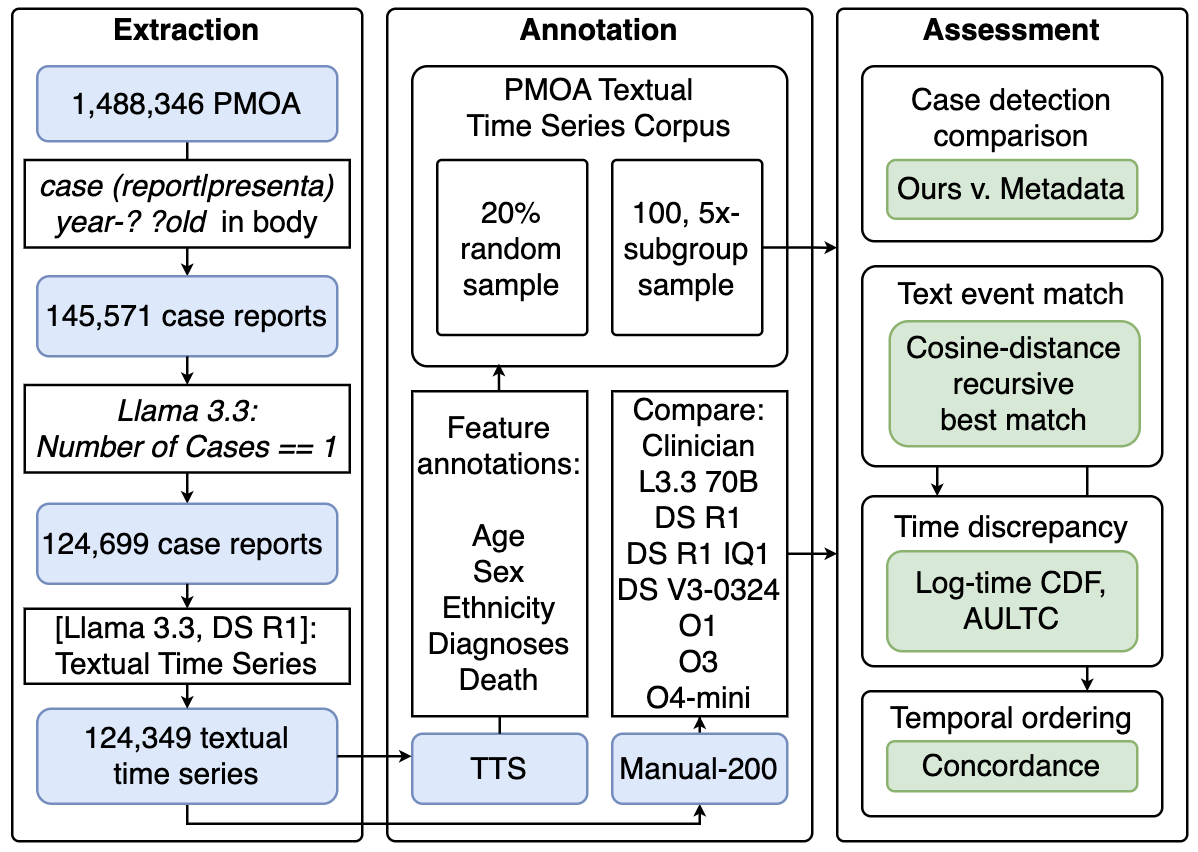
\includegraphics[width=0.75\linewidth]{Plots_tables/PMOATTS_flow5.png} % Adjust width
    \caption{Flowchart of the extraction and annotation pipeline. The left panel (Extraction) shows how we filtered the PMOA corpus to identify single-patient case reports. The middle panel (Annotation) depicts the generation of textual time series for each case via LLM prompting and the creation of evaluation subsets. The right panel (Assessment) summarizes the evaluation process, including metadata comparison, text event matching, time discrepancy analysis (log-time CDF, AULTC), and temporal order concordance.
    }
    \label{fig:flowchart}
    \vspace{-2.5mm}
\end{figure}

\subsection{Case Report Identification Pipeline}
\label{sec:case-report-identification-pipeline}

We use the PubMed Open Access (PMOA) repository data, which includes 1.4 million published manuscripts. Specifically, we utilize the plain text files from the December 17, 2024 release, located in the \texttt{oa\_noncomm} folder, which supports both noncommercial and commercial use. Following our previous work in \cite{wang2025large}, we identify candidate case reports by extracting content between the section markers ``\texttt{==== Body}'' and ``\texttt{==== Ref}'', which separate the main text and references in the PMOA format.

To ensure relevance, we first filter documents by matching the body text with the regular expressions ``\texttt{(case report|case presentation}'' and ``\texttt{year-? ?old}''.
%\textcolor{red}{George: In the regular expression "(case report|case presenta)" -- why "presenta"? If this is not a typo, it would be helpful to explain the reasoning here?}.
This filter yields 145,571 candidate documents likely to be case reports or case series. To narrow this set to single-patient case reports, we use a large language model (\texttt{Llama 3.3 70B Instruct}) to analyze each document's body text. The model is prompted with: ``\texttt{You are a physician. Determine the number of case reports in the following manuscript. Return 0 if it is not a case report. Reply only with the number and nothing else.}'', followed by the document body. We retain documents for which the model replies with \texttt{1} and discard others. This two-stage process results in a final dataset of 124,699 single-patient case reports (Figure~\ref{fig:flowchart}).

We compared our LLM-based case report identification method with PubMed's metadata-based labeling using a carefully designed benchmark. We created a dataset of 100 reports across five diagnoses—Diabetes, Sepsis, Hypertension, COVID-19, and Atrial Fibrillation—with 10 reports per diagnosis from each method. A clinician manually reviewed and labeled each report to verify whether it described exactly one case. 
%\textcolor{red}{Our LLM-pipeline significantly outperforms PubMed metadata filtering, particularly in terms of specificity and precision.}

%%%%%%%%%%%%%%%%%%%%%%%%%%%%
%%%%%%%%%%%%%%%%%%%%%%%%%%%%

\subsection{Timeline Annotation via LLM Prompting}
\label{sec:timeline-annotation}

\subsubsection{Textual Time Series (TTS)}
\label{sec:textual-time-series}

We used LLMs (\texttt{Llama 3.3 70B}, \texttt{DeepSeek-R1}) to extract clinical textual time series from PMOA case reports. A textual time series is a chronologically ordered sequence of clinical findings, each associated with a timestamp and a specific patient. A clinical finding refers to a free-text description of a health-related condition affecting the patient. Our approach differs from conventional \jeremy{'conventional' vague; word choice? tagging/span-based?} methods (e.g., \cite{sun2013evaluating, uzuner20112010}) by capturing longer, more context-rich text spans to accurately convey the meaning of clinical findings. Unlike the i2b2 guidelines, we do not limit findings to short prepositional phrases. For example, ``pain in chest that radiates substernally'' is kept intact to preserve its clinical nuance. Additionally, conjunctive findings are separated for clarity—e.g., ``metastases in the liver and pancreas'' is split into ``metastasis in the liver'' and ``metastasis in the pancreas.'' \jeremy{Can we be more specific about (syntax and) semantics? Syntax: list of free text spans, each associated with a numeric value indicating hours from case presentation. Semantics: What is our definition of an event ``clinical finding''; above, what constitutes a ``condition''; are age, sex, sociodemographics a 'conditions'? What is not a condition? Likewise what is our definition of the timing? For example, having defined TTS the task is not to output any valid TTS. What TTS are we requesting? Also, how do we address natural language descriptions of time intervals. For natural language specifications of temporal uncertainty, what is chosen? Once these are clarified, how do we actualize the process of getting from case report to textual time series (reflected in the prompt?)? Some of this is mentioned as in the prompt crafting, but I would suggest that the specification should be declared and then the prompt is an attempt to achieve that spec.}

To construct clinical textual time series, we adopt the LLM extraction prompt from previous work \citep{wang2025large,noroozizadeh2025reconstructing}. This prompt instructs the LLM to extract clinical events with timestamps, setting the admission event at a reference time of 0, with other events expressed in relative hours (negative for pre-admission events, positive for post-admission). It also provides guidelines for handling conjunctions, event durations, and output formatting. \textcolor{blue}{Full prompt for extracting TTS from case reports are in Supplementary Material Section~\ref{apd:extraction-prompt}.}

%\input{Scientific_data/Supplementary/TTS_extraction_prompt}

For each report, the LLM generates a structured sequence of \mbox{(clinical event, time)} tuples. Events are retained in free-text form to preserve their clinical specificity, rather than being mapped to a fixed ontology. On average, each report contains 46 events, with significant variation depending on report length and complexity. The corpus as a whole includes over 5.6 million timestamped events, making it the largest public dataset of its kind in clinical NLP. 

\subsubsection{Gold Standard Annotations}
\label{sec:gold-standard-annotations}

We constructed a gold-standard reference set of 200 manually annotated case reports, consisting of 180 cases randomly sampled from PMOA–TTS and 20 cases from our prior pilot study. All annotations were performed by a single clinical expert following a detailed annotation guideline designed to preserve fidelity to the original narrative while producing event representations suitable for temporal evaluation.

Annotators marked exact text spans corresponding to clinical events without rewriting or paraphrasing, with a small number of controlled exceptions specified in the guideline. First, conjunctive findings (e.g., “nausea and vomiting”) were permitted to be split into individual events when clinically meaningful. Second, when needed to supply context, annotators could prepend short clarifying phrases such as “history of” to ensure that extracted events were interpretable as stand-alone findings. Beyond these two exceptions, events were expected to remain faithful to the wording and granularity of the source text.

To ensure consistency, the guideline required that each event be able to stand alone semantically (e.g., distinguishing “SCC of the lung” rather than simply “SCC” \jeremy{to disambiguate from other anatomical lesions such as squamous cell carcinoma of the skin or sickle cell crisis}), that related findings be disambiguated when necessary, and that duplication of the same event be avoided when it appeared in multiple parts of the note. Pertinent negative or termination events (e.g., “no shortness of breath”, “denies chest pain”) were included when explicitly stated. These conventions were applied uniformly across the 200 reports.

Each annotated event was assigned a timestamp relative to a standardized case reference point. By definition, this reference point was the time of admission. In the rare cases \jeremy{either remove "rare" or quantify} where an explicit admission time was not stated, the encounter date (the earliest unambiguous point of clinical evaluation within the case narrative) was used as the reference time. For temporal expressions that described intervals, the start time of the interval was recorded. All timestamps were expressed in hours relative to the reference time (t=0).

These manually produced timelines serve as the reference standard for evaluating LLM-generated annotations in subsequent sections.

\subsection{Evaluation Metrics}
\label{sec:evaluation-metrics}

We assessed the textual time series extracted from PMOA case reports along three dimensions: (i) how well the extracted clinical events match up with manually annotated reference events (event match rate), (ii) how well the ordering of extracted clinical events matches that of the reference event ordering (temporal concordance), and (iii) how well extracted event times correspond to reference event times (time discrepancy). \textcolor{blue}{Formal definitions, implementation details, and sensitivity analyses for these metrics are provided in the Supplementary Material Sections~\ref{apd:evaluation-metrics} and \ref{apd:sensitivity-analyses} respectively.}

\begin{itemize}
    \item \textbf{\emph{Event match rate}} measures the proportion of manually annotated events that have a corresponding model-generated event within a predefined similarity threshold in embedding space, reflecting how many reference events are successfully recovered.
    \item \textbf{\emph{Temporal concordance}} (c-index) evaluates whether the relative ordering of event times in the model output agrees with the manually annotated timelines, providing a order-based summary of temporal consistency.
    \item \textbf{\emph{Log-time discrepancy}} quantifies the absolute difference between the log-transformed timestamps of matched events, and we summarize its distribution using the Area Under the Log-Time CDF (AULTC), which captures the cumulative proportion of events achieving small timing errors.  
\end{itemize}

%All LLM annotation, validation, and downstream survival experiments were run on Linux servers equipped with recent NVIDIA GPUs. Approximate GPU-hours by model, together with hardware specifications and runtime breakdowns, are reported in the Supplementary Information to facilitate reproducibility and cost estimation.


%%%%%%%%%%%%%%%%%%%%%%%%%%%%%%%%%%%%%%%%%
%%%%%%%%%%%%%%%% Data Records %%%%%%%%%%%%
%%%%%%%%%%%%%%%%%%%%%%%%%%%%%%%%%%%%%%%%

\section{Data Records}
\label{sec:data-records}

The PMOA–TTS dataset is hosted on Hugging Face Datasets at \url{https://huggingface.co/datasets/snoroozi/pmoa-tts} and is released under \textbf{CC BY-NC-SA 4.0}. The dataset card lists task tags (\texttt{Text Classification, Time Series Forecasting}), modality (\texttt{Text}), format support (\texttt{Parquet via auto-conversion}), language (\texttt{English}), and size (“\texttt{100K–1M}”). Data record schema with an example JSON entry is shown in Figure~\ref{fig:record_schema}. PMOA-TTS has the following dataset splits: 

\input{Scientific_data/Supplementary/data_records_json_table}

%\subsection{Dataset Splits}
\begin{itemize}
    \item \texttt{train\_DSR1/L33}: The full dataset of 125k single-patient case reports automatically extracted using and \texttt{DeepSeek-R1} and \texttt{Llama 3.3 70B} respectively. These are the default splits \jeremy{what does split refer to here} and contain the primary annotations used in downstream tasks.
    
    \item \texttt{case\_study\_100}: A curated benchmark of 100 case reports, used in the paper to evaluate LLM-based vs.\ metadata-based case report identification. Each sample has been manually reviewed for single-case validity \jeremy{what is ``single-case validity''? existence of exactly 1 case in the text?} across five different diagnoses.
    
    \item \texttt{case\_study\_25k\_L33}: A 25k-case subset of \texttt{Llama 3.3 70B}-annotated reports used for downstream survival analysis experiments in the paper. This split \jeremy{what does split refer to here? subset?} is designed to support modeling and evaluation of time-to-event outcomes on a more computationally manageable subset.
    
    \item \texttt{case\_study\_25k\_DSR1}: A 25k-case subset of \texttt{DeepSeek-R1}-annotated reports (same case reports corresponding to \texttt{case\_study\_25k\_L33})used for downstream survival analysis experiments. The \texttt{textual\_timeseries} and \texttt{death\_info} fields in this split are reconstructed from \texttt{DeepSeek-R1} outputs, enabling comparative analysis between models across an identical patient cohort.
    
    \item \texttt{case\_study\_n200}: A benchmark of 200 manually reviewed case reports used for qualitative and quantitative evaluation of LLM-generated annotations. Each model is evaluated across five independent runs on this subset to assess run-to-run variability in annotation consistency.

    %\item Model-specific splits for the \texttt{case\_study\_n200} subset include: (i) \texttt{Manual Annotations}, (ii) \texttt{DeepSeek-V3-0324}, (iii) \texttt{Llama 3.3 70B}, (iv) \texttt{OpenAI O1}, (v) \texttt{OpenAI O3}, (vi) \texttt{OpenAI O4-mini} and (vii) \texttt{OpenAI GPT5}. These model-specific splits each contain outputs from $5$ different runs for each model for the same set of 200 manually annotated case reports.
\end{itemize}

The data repository also has an additional data split \texttt{TTS\_n200\_additional\_models}, which bundles the single-expert manual timelines (the reference set) together with parallel LLM-generated textual time series for additional models, including open-weight models such as \texttt{DeepSeek-V3}, \texttt{DeepSeek-R1 quantized}, and \texttt{DeepSeek-V3-0324}, and proprietary OpenAI models such as \texttt{GPT5}, \texttt{O1}, \texttt{O3}, and \texttt{O4-mini}. This split is designed for lightweight benchmarking and cross-model comparison on a fixed 200-case cohort without re-annotating the full corpus. For the full 125k release, we provide textual time series produced by \texttt{DeepSeek-R1} and \texttt{Llama 3.3 70B}; the additional models are released only on the 200-case subset due to resource constraints. For completeness, both \texttt{Llama 3.3 70B} and \texttt{DeepSeek-R1} were also executed in five independent runs on the \texttt{case\_study\_n200} subset, and these annotated outputs are included in the dataset.


%%%%%%%%%%%%%%%%%%%%%%%%%%%%%%%%%%%%%%%%%
%%%%%%%%%%%%%%%% Data Overview
%%%%%%%%%%%%%%%%%%%%%%%%%%%%%%%%%%%%%%%%

\section{Data Overview}
\label{sec:data-overview}

\subsection{Cohort Demographics}
\label{sec:cohort-demographics}

For demographic extraction, we used an LLM-based query to retrieve age, sex, and ethnicity for each case. 
The prompt instructed the model to report age in years; sex as \texttt{Male}, \texttt{Female}, a free-text category, or \texttt{Not Specified}; and ethnicity according to U.S.\ Census categories or \texttt{Not Specified} (\textcolor{blue}{full prompt in Supplementary Material Section~\ref{apd:demographics-prompt}}).

Across PMOA--TTS, the median age is 47 years, with peaks at 5-year intervals, consistent with rounded age reporting in clinical text (Figure~\ref{fig:demo}). 
The inferred sex distribution is approximately balanced (52\% male, 47\% female, 1\% not specified). 
Ethnicity is rarely documented: 89\% of case reports lack explicit ethnicity, and among those that do, White/Caucasian (5\%) and Asian (3\%) are most common, followed by African (1\%) and Other (2\%). 
The relative enrichment of Asian patients likely reflects the international authorship of PubMed case reports rather than any single healthcare system.

\input{Scientific_data/Supplementary/age_fig_demo_table}

\subsection{Descriptive Statistics}
\label{sec:descriptive-statistics}

The textual time series (TTS) derived from case reports show substantial variation in sequence length and temporal span. 
On average, each TTS contains $\sim 46$ timesteps \jeremy{mean? median?}, with 50\% of sequences comprising between 33 and 57 timesteps (Figure~\ref{fig:tts_stats}a). 
The length distribution is right-skewed, with a small number of very long trajectories exceeding $1{,}000$ timesteps. 
Events are generally concise: the mean event span is 3.6 words (26.1 characters), and most events fall between two and five words, such as \texttt{“admitted to the hospital”} or \texttt{“CT scan performed”}. 
Longer spans (e.g., $\geq 15$ words) typically correspond to detailed histopathologic or imaging descriptions.

The temporal coverage of individual case reports also varies widely. 
The mean case duration is 415.9 days (median 104.0 days), with half of cases spanning between 28 and 391 days and the 99th percentile extending to 4{,}380 days (12 years). 
On average, 77.6\% of events share timestamps with at least one other event, indicating frequent temporal co-occurrence within a report. 
The median uniqueness ratio of event timestamps is 0.14, reflecting the common practice of documenting multiple events at the same recorded time (e.g., grouped laboratory results or procedure bundles). 
Approximately 17\% of events have negative timestamps, representing history prior to the chosen reference point (typically admission), such as past diagnoses or prior treatments.
Together, these statistics summarize the density and temporal heterogeneity of clinical event sequences across PMOA--TTS. 
}
\vspace{-5mm}
\begin{figure}[!htbp]
    \centering
    \begin{minipage}{0.48\textwidth}
        \centering
        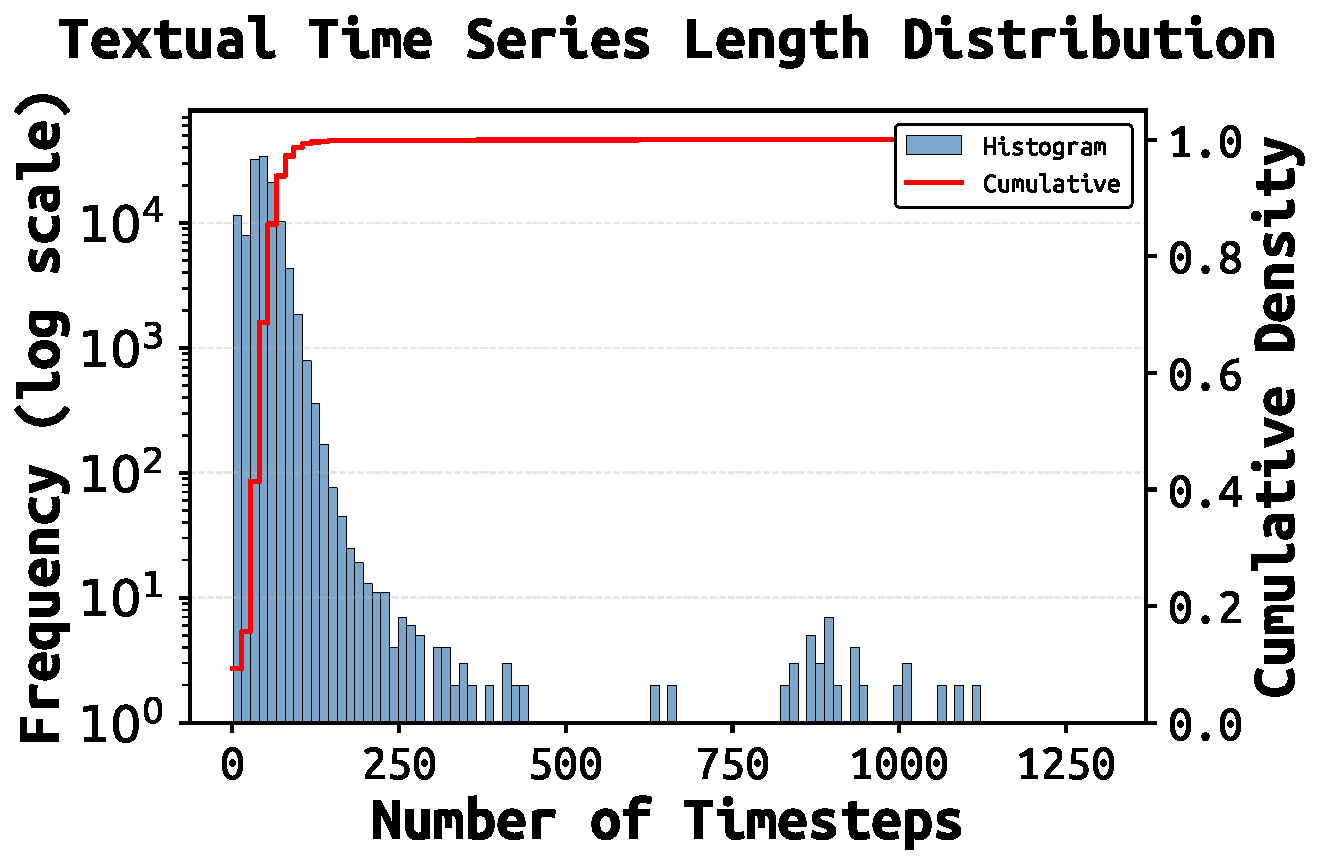
\includegraphics[width=\linewidth]{Plots_tables/tts_length_distribution.pdf}
        \caption*{(a) Distribution of time series lengths (timesteps) across the dataset.}
    \end{minipage}\hfill
    \begin{minipage}{0.48\textwidth}
        \centering
        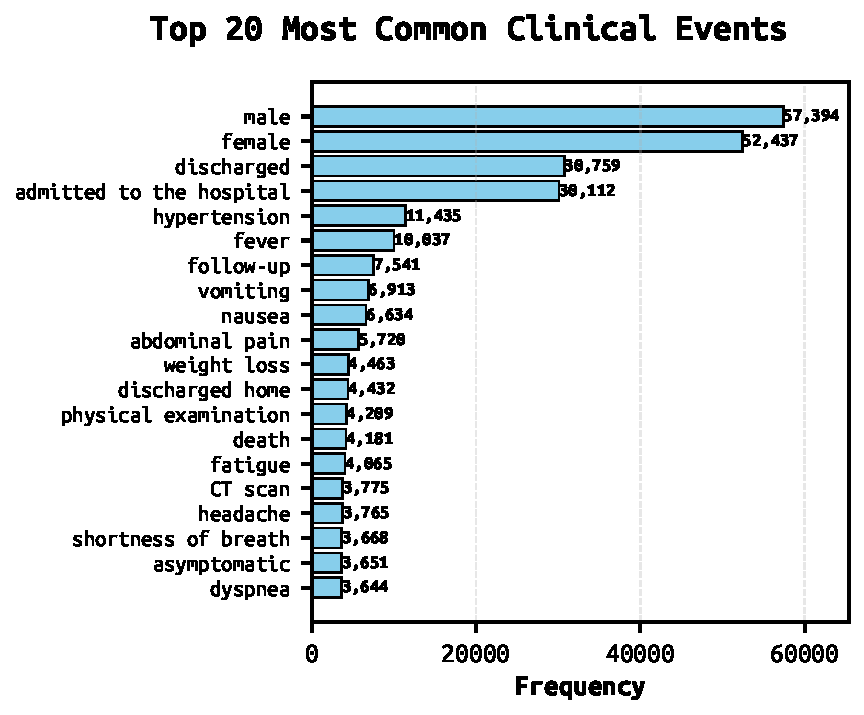
\includegraphics[width=\linewidth]{Plots_tables/top_20_common_events.pdf}
        \caption*{(b) Most frequently occurring events across all case reports.
        \textcolor{red}{Jeremy: Not sure why the male/female count sums to about 110k, from a cohort of 124k.}}
    \end{minipage}
    \caption{Overview of textual time series characteristics in PMOA--TTS.}
    \label{fig:tts_stats}
    \vspace{-7.5mm}
\end{figure}

\subsection{Diagnosis Distribution Analysis}
\label{diagnosis-distribution-analysis}

To characterize diagnostic coverage, we prompted the LLM to act as an expert physician and list patient-specific diagnoses for each case report. 
The prompt asked the model to extract final diagnostic labels (e.g., ``acne'', ``DRESS syndrome'') rather than isolated clinical findings (e.g., ``rash'', ``leukocytosis''), to place the primary diagnosis first, and to output one diagnosis per line without explanatory text (\textcolor{blue}{full prompt in Supplementary Material Section~\ref{apd:diagnosis-prompt}}).

Free-text diagnoses were then standardized to the Unified Medical Language System (UMLS) using the ScispaCy entity linker (\texttt{en\_core\_sci\_lg}) with the UMLS knowledge base. 
For each extracted diagnosis, we selected the highest-ranked UMLS concept under a high-confidence threshold, and retrieved its canonical name for downstream analysis (\textcolor{blue}{for further details, refer to Supplementary Material Section~\ref{apd:umls-mapping})}.

Figure~\ref{fig:top_diagnoses} shows the 20 most frequent UMLS-normalized diagnoses in PMOA--TTS. 
These are dominated by common cardiometabolic and renal conditions, including hypertensive disorders (e.g., essential hypertension, systolic and diastolic hypertension), diabetes mellitus and its subtypes, and chronic kidney disease. 
Thus, the most frequently observed diagnoses align with high-prevalence chronic diseases in middle-aged and older adults, consistent with the cohort's age distribution.

We further examined co-occurrence structure using a clustered heatmap of diagnosis pairs (Figure~\ref{fig:diagnosis_cooccurrence}). 
The heatmap reveals coherent clusters of related conditions, such as hypertensive disorders, diabetes variants, and chronic kidney disease, as well as groupings linking cardiovascular and metabolic diagnoses. 
These patterns recapitulate well-established comorbidity relationships (e.g., diabetes with nephropathy, or atrial fibrillation with hypertension) and illustrate how the corpus captures clinically meaningful disease constellations. 
% While the top diagnoses reflect modal cardiometabolic conditions, the full set of mapped concepts spans a broader range of organ systems and disease categories (see Supplementary Tables for extended distributions and rare-condition coverage).

\vspace{-5mm}
\begin{figure}[!htbp]
    \centering
    \begin{subfigure}[t]{0.39\textwidth}
        \centering
        \raisebox{40pt}{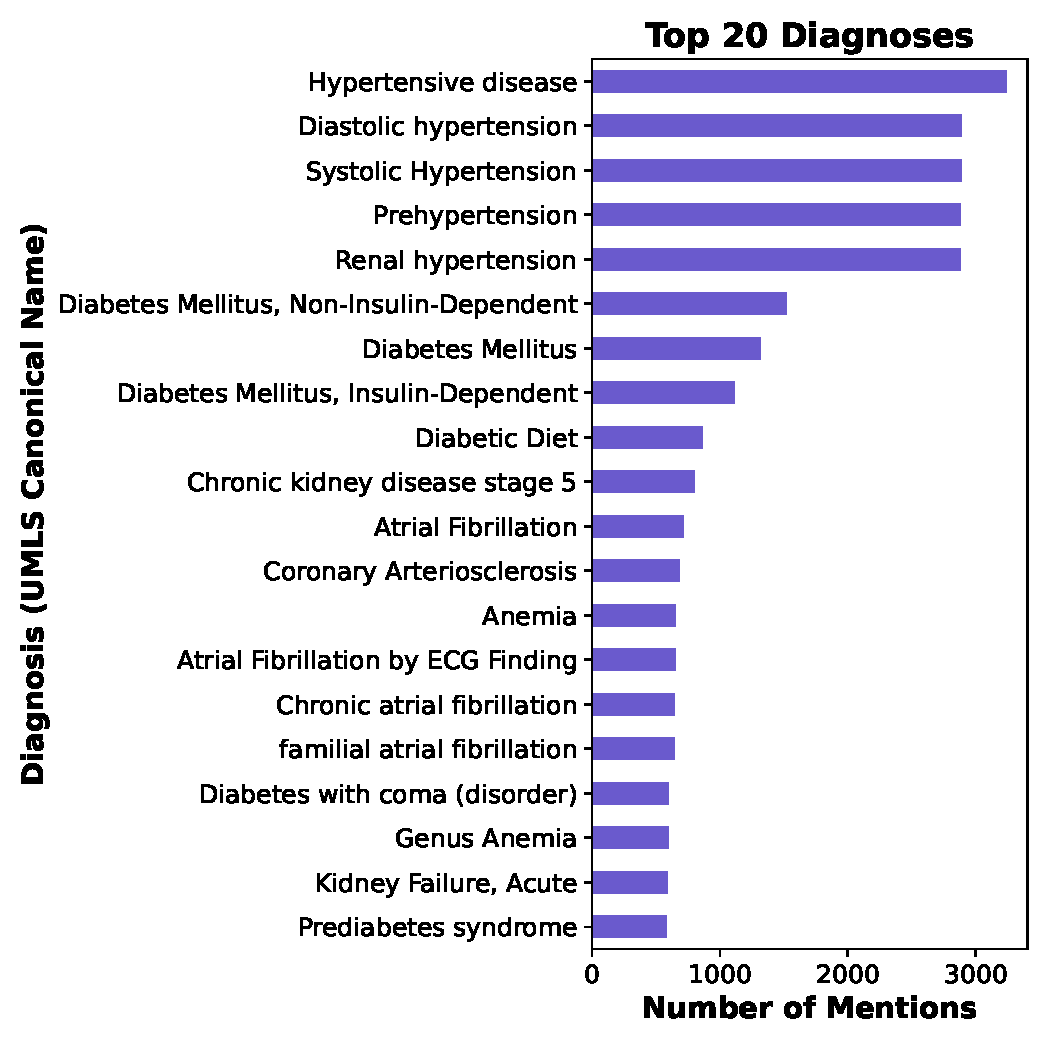
\includegraphics[width=0.99\linewidth]{Plots_tables/top_diagnoses_umls.pdf}}
        \caption{Most frequent diagnoses.}
        \label{fig:top_diagnoses}
    \end{subfigure}
    \hfill
    \begin{subfigure}[t]{0.6\textwidth}
        \centering
        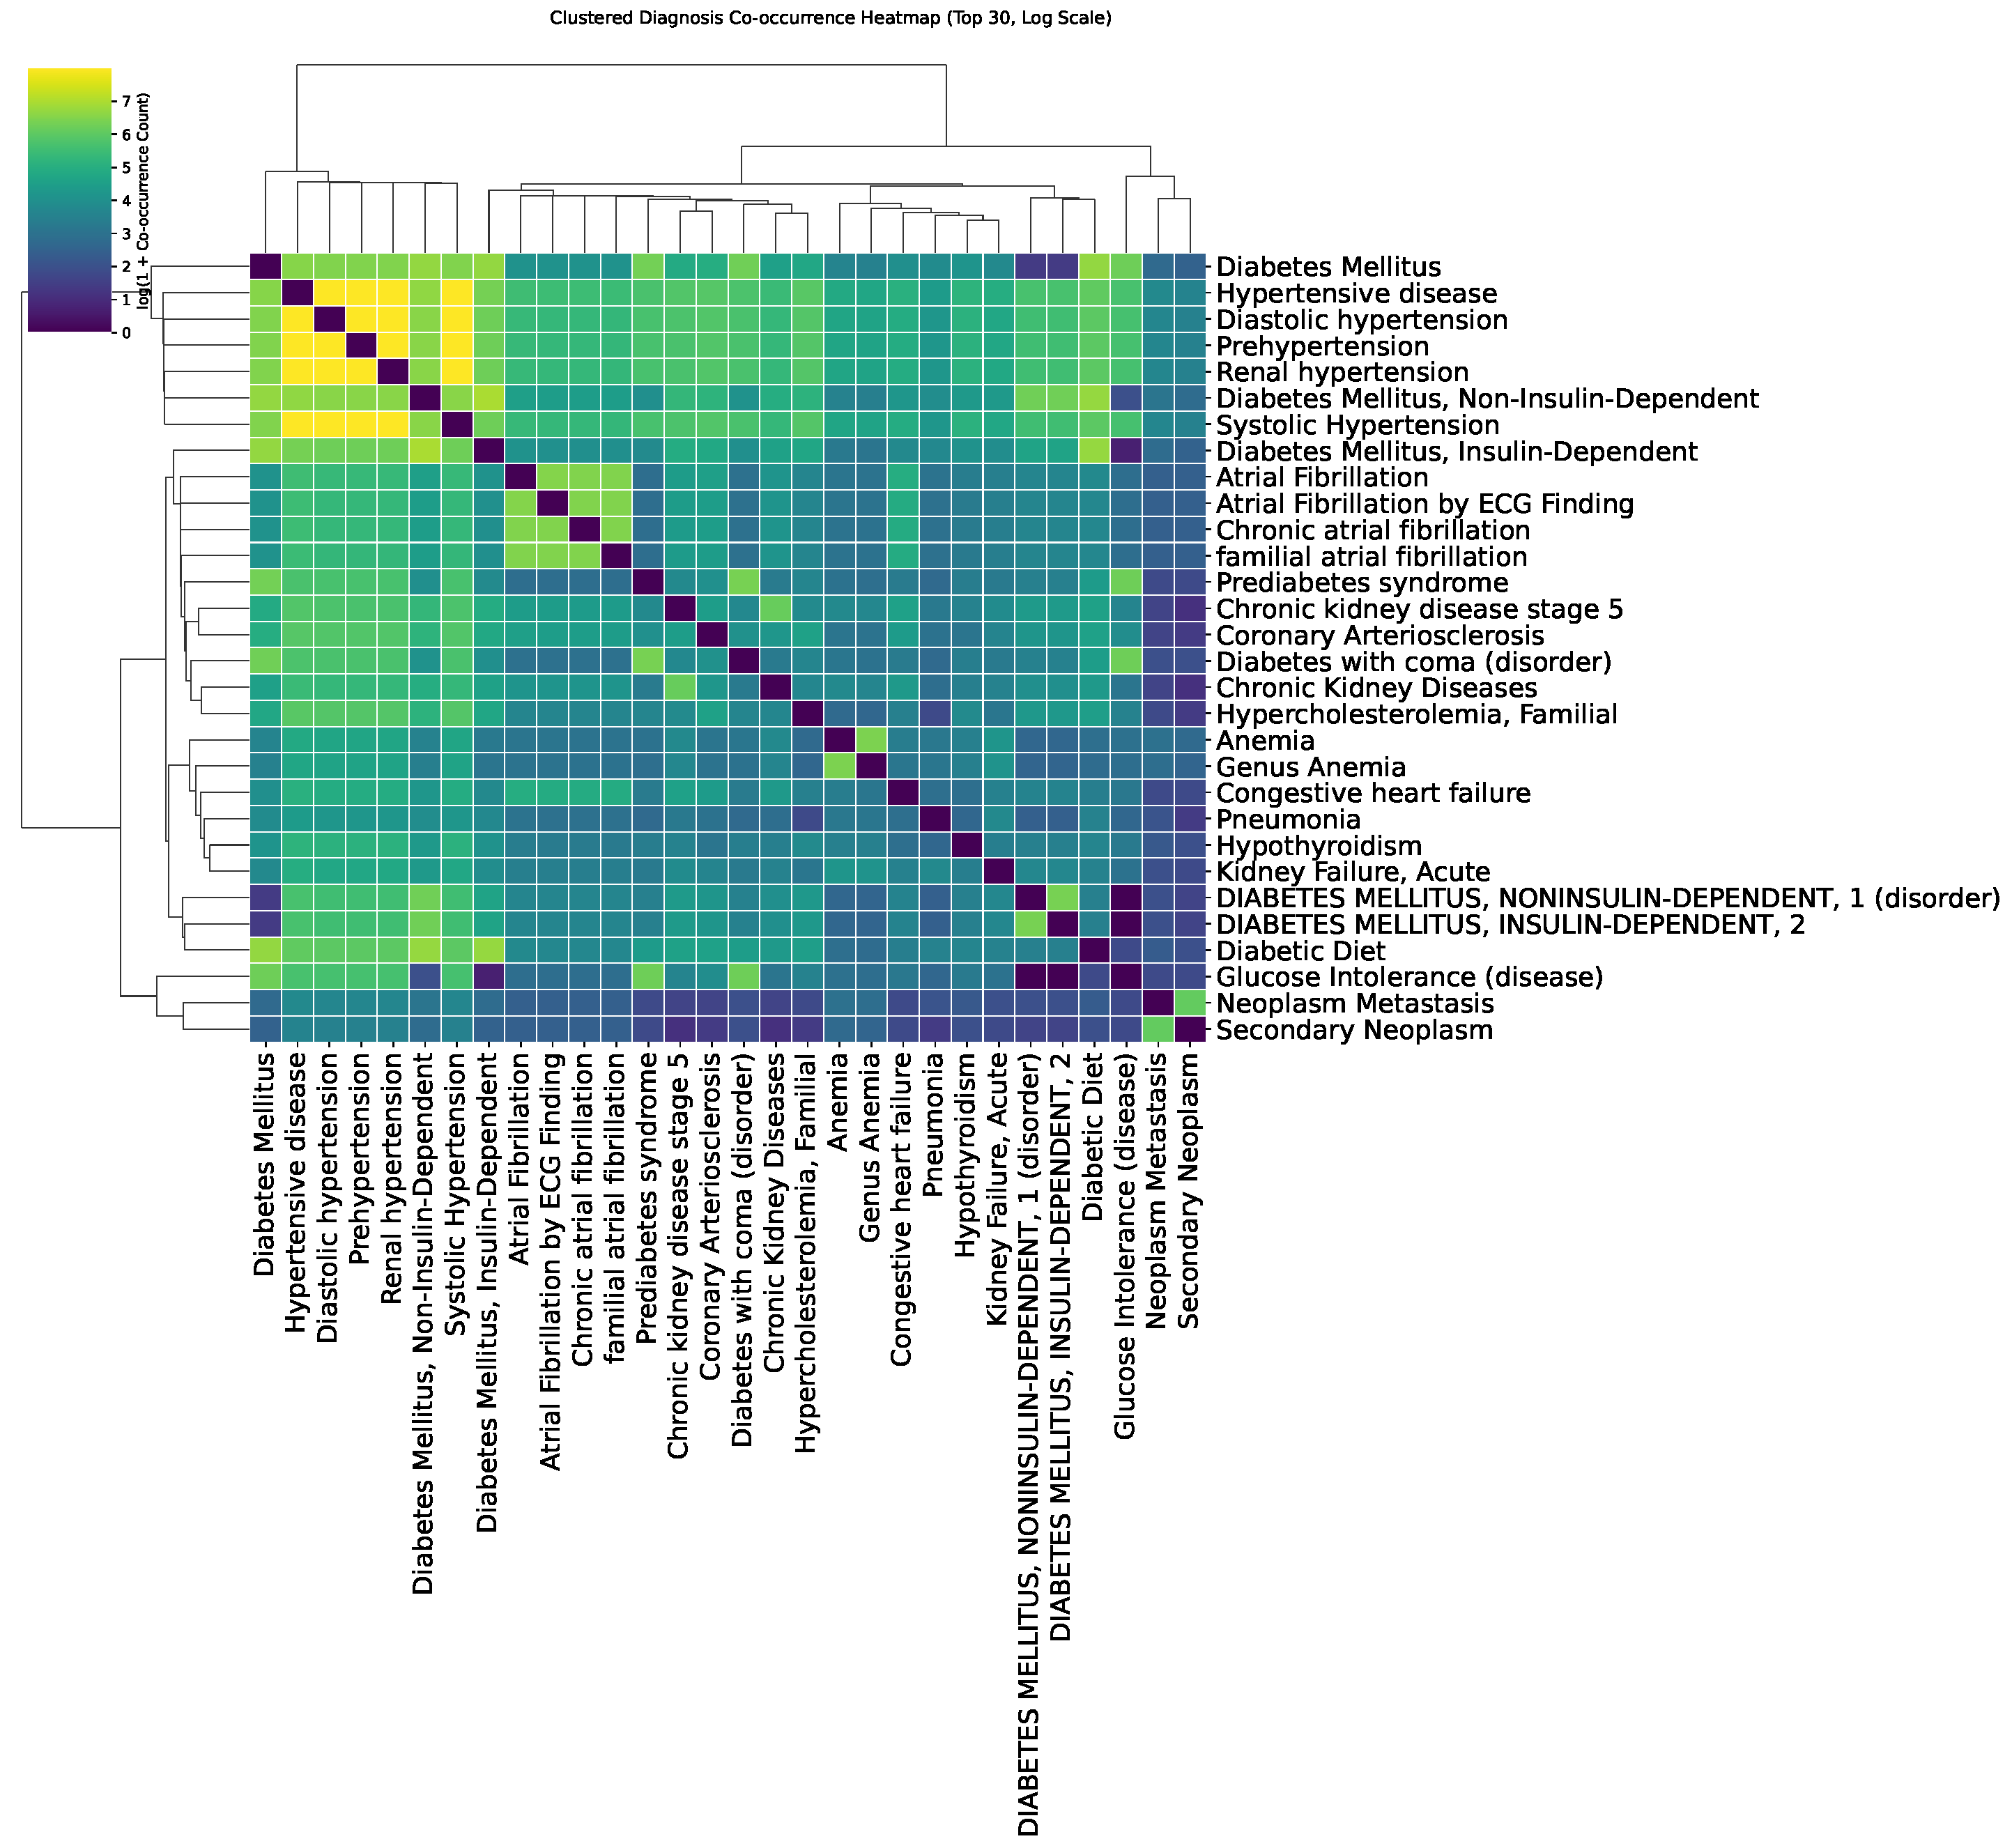
\includegraphics[width=0.99\linewidth]{Plots_tables/clustered_cooccurrence_heatmap_top30.pdf}
        \caption{Diagnosis co-occurrence heatmap.}
        \label{fig:diagnosis_cooccurrence}
    \end{subfigure}
    \caption{Frequency and co-occurrence patterns of UMLS-normalized diagnoses in PMOA--TTS. 
    The left panel shows the 20 most frequently mentioned diagnoses using canonical UMLS names. 
    The right panel visualizes pairwise co-occurrence (log-transformed counts) among common diagnoses, with hierarchical clustering highlighting groups of frequently co-mentioned conditions. \jeremy{can we get prevalence of disease (groups) to compare them with general prevalence rates from other data sources? That would give better point of comparison (and possibly illustrate degree to which it overemphasizes rare/atypical cases) and communicate more information than "yes we see the top diagnoses showing up in our dataset".}}
    \label{fig:diagnoses}
    \vspace{-7.5mm}
\end{figure}

%%%%%%%%%%%%%%%%%%%%%%%%%%%%%%%%%%%%%%%%%%%%%%%%
%%%%%%%%%%%%%%%%% Technical validation %%%%%%%%%%%
%%%%%%%%%%%%%%%%%%%%%%%%%%%%%%%%%%%%%%%%%

\section{Technical Validation}
\label{sec:technical-validation}

\subsection{Case Report Identification Performance}
\label{sec:case-report-identification-performance}

\begin{table}[t!]
\footnotesize
\centering
\caption{\rebuttal{Case-report identification performance by diagnosis and in aggregate on the manually reviewed 100-document evaluation set. Recall is calculated with respect to confirmed single-patient case reports within this evaluation set.}}
\label{tab:case_report_identification}
% \begin{adjustbox}{max width=0.95\textwidth}
\begin{tabular}{llcccc}
\toprule
Subset & Diagnosis & Precision & Recall & Accuracy & F1 Score \\
\midrule
\multirow{6}{*}{PubMed metadata} 
    & Atrial Fibrillation & 0.84 & 0.94 & 0.80 & 0.89 \\
    & COVID-19            & 0.94 & 0.89 & 0.85 & 0.92 \\
    & Diabetes            & 0.85 & 1.00 & 0.85 & 0.92 \\
    & Hypertension        & 1.00 & 1.00 & 1.00 & 1.00 \\
    & Sepsis              & 0.95 & 0.95 & 0.90 & 0.95 \\
\cmidrule(lr){2-6}
    & \textbf{All Diagnoses} & \text{0.92} & \textbf{0.96} & \text{0.88} & \text{0.94} \\
\midrule
\multirow{6}{*}{LLM-Pipeline}
    & Atrial Fibrillation & 1.00 & 1.00 & 1.00 & 1.00 \\
    & COVID-19            & 1.00 & 0.89 & 0.90 & 0.94 \\
    & Diabetes            & 1.00 & 0.94 & 0.95 & 0.97 \\
    & Hypertension        & 1.00 & 0.95 & 0.95 & 0.97 \\
    & Sepsis              & 1.00 & 1.00 & 1.00 & 1.00 \\
\cmidrule(lr){2-6}
    & \textbf{All Diagnoses} & \textbf{1.00} & \textbf{0.96} & \textbf{0.96} & \textbf{0.98} \\
\bottomrule
\end{tabular}
% \end{adjustbox}
\vspace{-5mm}
\end{table}



% \begin{table}[!ht]
%     \footnotesize
%     \centering
%     \caption{Case report identification performance per diagnosis}
%     \label{tab:diagnosis_results}
%     \begin{tabular}{l l c c c c c}
%         \hline
%         Subset & Diagnosis & Sensitivity & Specificity & Accuracy & Precision & F1 Score \\
%         \hline
%         PubMed MetaData  & Atrial Fibrillation & 0.94 & 0.00 & 0.80 & 0.84 & 0.89 \\
%         LLM-Pipeline     & Atrial Fibrillation & 1.00 & 1.00 & 1.00 & 1.00 & 1.00 \\
%         \hline
%         PubMed MetaData  & COVID-19           & 0.89 & 0.00 & 0.85 & 0.94 & 0.92 \\
%         LLM-Pipeline     & COVID-19           & 0.89 & 1.00 & 0.90 & 1.00 & 0.94 \\
%         \hline
%         PubMed MetaData  & Diabetes           & 1.00 & 0.00 & 0.85 & 0.85 & 0.92 \\
%         LLM-Pipeline     & Diabetes           & 0.94 & 1.00 & 0.95 & 1.00 & 0.97 \\
%         \hline
%         PubMed MetaData  & Hypertension       & 1.00 & 0.00 & 1.00 & 1.00 & 1.00 \\
%         LLM-Pipeline     & Hypertension       & 0.95 & 0.00 & 0.95 & 1.00 & 0.97 \\
%         \hline
%         PubMed MetaData  & Sepsis             & 0.95 & 0.00 & 0.90 & 0.95 & 0.95 \\
%         LLM-Pipeline     & Sepsis             & 1.00 & 1.00 & 1.00 & 1.00 & 1.00 \\
%         \hline
%     \end{tabular}
% \end{table}

% \begin{table}[!ht]
%     \footnotesize
%     \centering
%     \caption{Aggregated case report identification performance across all diagnoses}
%     \label{tab:aggregated_results}
%     \begin{tabular}{l c c c c c}
%         \hline
%         Subset & Sensitivity & Specificity & Accuracy & Precision & F1 Score \\
%         \hline
%         PubMed MetaData  & \textbf{0.96} & 0.00 & 0.88 & 0.92 & 0.94 \\
%         LLM-Pipeline     & \textbf{0.96} & \textbf{1.00} & \textbf{0.96} & \textbf{1.00} & \textbf{0.98} \\
%         \hline
%     \end{tabular}
% \end{table}

We first evaluated the accuracy of identifying single-patient case reports using our LLM-based pipeline compared with a PubMed metadata filter across five diagnostic categories (diabetes, sepsis, hypertension, COVID-19, and atrial fibrillation). Using clinician-assigned labels on the \texttt{case\_study\_100} benchmark as ground truth, we computed precision, recall, accuracy, and F1 score for each approach (Table~\ref{tab:case_report_identification}). \jeremy{this seems like a methods paragraph}

In this evaluation set, the LLM-based pipeline achieved precision of 1.00 across all diagnostic categories and in aggregate, meaning that every document flagged as a single-patient case report by the pipeline was confirmed as such in this sample. The PubMed metadata filter showed lower and more variable precision, ranging from 0.84 (atrial fibrillation) to 1.00 (hypertension), with an overall precision of 0.92. Both methods achieved similar recall (0.96 overall), indicating comparable ability to recover true case reports.

Overall accuracy was higher for the LLM-based pipeline (0.96 vs.\ 0.88), largely due to better exclusion of multi-patient or non-case-report articles that were sometimes misclassified by the metadata-based filter. Performance patterns were consistent across diagnostic subsets, with the LLM pipeline maintaining high F1 scores (0.94–1.00). These results support the use of the LLM-based approach to construct a high-precision corpus of single-patient narratives for PMOA--TTS, while recognizing that performance is estimated on a finite, diagnosis-targeted benchmark.

\subsection{Evaluation of Clinical Textual Time Series Quality}
\label{sec:evaluation-of-tts-quality}

We next assessed the quality of the extracted textual time series using 200 manually annotated case reports as reference. Each large language model (LLM) annotator was evaluated across five independent runs to capture run-to-run variation in the generated timelines. For each model and run, we computed three complementary metrics: (i) event match rate (proportion of reference events with a semantically matched model event under a cosine distance threshold), (ii) temporal concordance (c-index) among matched events, and (iii) Area Under the Log-Time CDF (AULTC) summarizing timestamp alignment errors. \jeremy{this seems like a methods paragraph}

Table~\ref{tab:model_comparison} reports mean and standard deviation across runs for seven LLM variants: \texttt{Llama 3.3 70B}, \texttt{DeepSeek-R1}, \texttt{DeepSeek-V3-0324}, \texttt{OpenAI GPT5}, \texttt{OpenAI O4-mini}, \texttt{OpenAI O3}, and \texttt{OpenAI O1}. \texttt{OpenAI GPT5} achieves the highest mean match rate (0.847 $\pm$ 0.005), indicating the most comprehensive coverage of manually annotated events. \texttt{OpenAI O3} attains the highest concordance (0.891 $\pm$ 0.006), and \texttt{OpenAI O4-mini} yields the highest AULTC (0.748 $\pm$ 0.003), reflecting strong timestamp alignment among matched events. Standard deviations are generally small across runs, suggesting stable behavior for a given model.

\begin{table}[h!]
\vspace{-5mm}
\centering
\caption{Comparison of models on Match Rate, Concordance, and AULTC with respect to 200 manually annotated case reports across 5 independent runs for each model.}
\label{tab:model_comparison}
\begin{tabular}{lccc}
\hline
\textbf{Model} & \textbf{Match Rate} & \textbf{Concordance} & \textbf{AULTC} \\
\hline
\texttt{Llama 3.3 70B}       & 0.675 $\pm$ 0.003 & 0.835 $\pm$ 0.003 & 0.717 $\pm$ 0.001 \\
\texttt{DeepSeek-R1}         & 0.746 $\pm$ 0.008 & 0.785 $\pm$ 0.010 & 0.726 $\pm$ 0.003 \\
\texttt{DeepSeek-V3-0324}    & 0.761 $\pm$ 0.004 & 0.791 $\pm$ 0.005 & 0.728 $\pm$ 0.002 \\
\texttt{OpenAI GPT5}         & \textbf{0.847 $\pm$ 0.005} & 0.883 $\pm$ 0.002 & 0.719 $\pm$ 0.001 \\
\texttt{OpenAI O4-mini}      & 0.750 $\pm$ 0.019 & 0.842 $\pm$ 0.008 & \textbf{0.748 $\pm$ 0.003} \\
\texttt{OpenAI O3}           & 0.736 $\pm$ 0.003 & \textbf{0.891 $\pm$ 0.006} & 0.735 $\pm$ 0.003 \\
\texttt{OpenAI O1}           & 0.638 $\pm$ 0.007 & 0.880 $\pm$ 0.003 & 0.730 $\pm$ 0.001 \\
\hline
\end{tabular}
\vspace{-7.5mm}
\end{table}

\begin{table}[ht!]
\vspace{-7.5mm}
\centering
\caption{Bootstrap 95\% confidence intervals for Match Rate, Concordance, and AULTC across models evaluated on the 200 manually annotated case reports.\jeremy{suggest being consistent about number of sigfigs in results (see table 2)}}
\label{tab:bootstrap_intervals}
\begin{tabular}{lccc}
\hline
\textbf{Model} & \textbf{Match Rate (95\% CI)} & \textbf{Concordance (95\% CI)} & \textbf{AULTC (95\% CI)} \\
\hline
\texttt{Llama 3.3 70B}      & [0.6420, 0.7176] & [0.8333, 0.8611] & [0.7010, 0.7540] \\
\texttt{DeepSeek-R1}        & [0.6944, 0.7733] & [0.7825, 0.8175] & [0.7080, 0.7515] \\
\texttt{DeepSeek-V3-0324}   & [0.7269, 0.7905] & [0.7923, 0.8214] & [0.7178, 0.7581] \\
\texttt{OpenAI GPT5}        & [0.8047, 0.8661] & [0.8815, 0.8986] & [0.7056, 0.7498] \\
\texttt{OpenAI O4-mini}     & [0.6921, 0.7672] & [0.8263, 0.8515] & [0.7320, 0.7696] \\
\texttt{OpenAI O3}          & [0.6986, 0.7654] & [0.8879, 0.9062] & [0.7278, 0.7645] \\
\texttt{OpenAI O1}          & [0.5990, 0.6772] & [0.8719, 0.8952] & [0.7163, 0.7550] \\
\hline
\end{tabular}
\vspace{-7.5mm}
\end{table}

To quantify uncertainty from a complementary perspective, we also performed a bootstrap analysis based on resampling the 200 annotated cases with replacement and recomputing metrics to obtain 95\% confidence intervals. These intervals characterize variability arising from the composition of the reference set, whereas the across-run standard deviations reflect variability in model sampling. The full set of bootstrap intervals is reported in Figure~\ref{tab:bootstrap_intervals}.

% \begin{figure}[!tbp]
% \centering
%     \begin{minipage}[t]{0.242\textwidth}
%     \centering
%     \includegraphics[page=1, width=\linewidth]{Plots_tables/pmoa_updated_man_figs.pdf}
%     \end{minipage}
%     \hfill
%     \begin{minipage}[t]{0.242\textwidth}
%     \centering
%     \includegraphics[page=2, width=\linewidth]{Plots_tables/pmoa_updated_man_figs.pdf}
%     \end{minipage}
%     \hfill
%     \begin{minipage}[t]{0.242\textwidth}
%     \centering
%     \includegraphics[page=3, width=\linewidth]{Plots_tables/pmoa_updated_man_figs.pdf}
%     \end{minipage}
%     \hfill
%     \begin{minipage}[t]{0.242\textwidth}
%     \centering
%     \includegraphics[page=4, width=\linewidth]{Plots_tables/pmoa_updated_man_figs.pdf}
%     \end{minipage}
%     \caption{Comparison of different LLM for extracting temporal clinical events from case reports. From left to right: (\textbf{A}) event match cumulative distribution function, (\textbf{B}) concordance box plots, (\textbf{C}) time discrepancy from manual annotation timestamps among matched events (overall), and (\textbf{D}) time discrepancy disaggregated by clinician annotator timestamp (time from presentation). 
%     %\textcolor{red}{Have same figure for LAPJV?}
%     }
%     \label{fig:tts_evaluation}
%     \vspace{-10pt}
% \end{figure}



\begin{figure}[!tbp]
\centering

% First row: panels A and B
\begin{minipage}[t]{0.49\linewidth}
    \centering
    \includegraphics[
        page=1,
        width=0.8\linewidth
    ]{Plots_tables/pmoa_updated_man_figs.pdf}
\end{minipage}
\hfill
\begin{minipage}[t]{0.49\linewidth}
    \centering
    \includegraphics[
        page=2,
        width=0.8\linewidth
    ]{Plots_tables/pmoa_updated_man_figs.pdf}
\end{minipage}

\par\medskip

% Second row: panels C and D
\begin{minipage}[t]{0.49\linewidth}
    \centering
    \includegraphics[
        page=3,
        width=0.8\linewidth
    ]{Plots_tables/pmoa_updated_man_figs.pdf}
\end{minipage}
\hfill
\begin{minipage}[t]{0.49\linewidth}
    \centering
    \includegraphics[
        page=4,
        width=0.8\linewidth
    ]{Plots_tables/pmoa_updated_man_figs.pdf}
\end{minipage}

\caption{
Comparison of different LLMs for extracting temporal clinical events
from case reports:
(\textbf{A}) cumulative distribution of event-matching cosine distances;
(\textbf{B}) temporal-concordance box plots;
(\textbf{C}) timestamp discrepancies between model-generated and manual
annotations among semantically matched events; and
(\textbf{D}) timestamp discrepancies stratified by the clinician-annotated
time relative to presentation.
}
\label{fig:tts_evaluation}
\vspace{-10pt}
\end{figure}


\subsubsection{Text Event Match Performance}
\label{sec:text-event-match-performance}
Figure~\ref{fig:tts_evaluation} (A) shows the cumulative distributions of cosine distances between model-generated and reference event descriptions, using a threshold of 0.1 to define a match. \texttt{DeepSeek-R1} and its quantized variant \texttt{DeepSeek-R1-UD-IQ1} exhibit the highest semantic alignment, with roughly 80\% of matched events falling below the threshold. \texttt{DeepSeek-V3-0324} and \texttt{O4-mini} form a second tier, while \texttt{Llama 3.3 70B}, \texttt{O1}, and \texttt{O3} display more dispersed similarity distributions. These results highlight meaningful differences in how effectively models capture the wording and semantics of clinical event mentions.

\subsubsection{Temporal Ordering Performance}
\label{sec:temporal-ordering-performance}
Using the same similarity threshold to identify matched events, temporal ordering accuracy was assessed via the concordance index (c-index). As shown in Figure~\ref{fig:tts_evaluation} (B), \texttt{Llama 3.3 70B} achieves the highest median c-index (0.96\jeremy{Is this a typo? I don't see the correspondence to the Figure}), followed closely by \texttt{DeepSeek-V3-0324} and \texttt{DeepSeek-R1}. Models with stricter matching behavior may obtain higher concordance by evaluating only confidently aligned events, whereas models with broader coverage face a more challenging ordering task. Notably, \texttt{Llama 3.3 70B} attains strong ordering performance despite a lower match rate, suggesting that when it aligns with reference events, it preserves relative timing well. \jeremy{guessing this paragraph needs refreshing}

\subsubsection{Time Discrepancy Analysis}
\label{sec:time-descrepancy-analysis}
Figure~\ref{fig:tts_evaluation} (C, D) also presents log-scaled time-discrepancy curves comparing predicted and reference timestamps. \texttt{DeepSeek-R1} shows the steepest cumulative curve, indicating closer absolute agreement with manual timestamps, while \texttt{Llama 3.3 70B} exhibits greater dispersion. Performance declines for all models as events occur farther from the admission reference time, as shown in the interval-stratified panel of Figure~\ref{fig:tts_evaluation}. Across patient timelines, \texttt{DeepSeek} models yield more accurate timestamping, whereas \texttt{Llama 3.3 70B} provides stronger relative ordering. Taken together, these analyses show that semantic matching, temporal ordering, and timestamp precision capture complementary aspects of textual time series quality.


\subsubsection{Additional Sensitivity Analyses}
\label{sec:additional-sensitivity-analyses}

% We conducted additional sensitivity analyses to probe robustness of the evaluation. Varying the event match distance threshold revealed expected trade-offs between event coverage and temporal performance (concordance and AULTC); very strict thresholds yield fewer but cleaner matches, whereas more permissive thresholds increase coverage at the cost of noisier ordering and timing (\textcolor{blue}{Supplementary Material Section 4.1 Figure 1}). We also examined the impact of prompt design on annotation quality, finding that structured prompts with explicit temporal instructions outperform zero-shot prompting and ablations that remove key guidance components (\textcolor{blue}{Supplementary Material Section 4.2 Figure 2}).

\paragraph{Varying the Event Match Distance Threshold}
We conducted sensitivity analyses to assess robustness with respect to the event match threshold. As expected, stricter thresholds produce fewer but cleaner matches, while more permissive thresholds increase coverage at the expense of noisier ordering and timing. Varying the cosine distance threshold from 0.01 to 0.25, we observed corresponding shifts in match rate, concordance, and AULTC. A threshold of 0.1 was chosen based on manual review of \texttt{Llama 3.3 70B Instruct} and \texttt{O1} outputs. The resulting trade-offs are summarized in Figure~\ref{fig:threshold_temporal_tradeoff}.

\paragraph{Sensitivity to Parts of the LLM Prompt Being Changed}
We conducted sensitivity analyses to assess how different components of the extraction prompt affect timeline quality (\textcolor{blue}{Supplementary Material Section~\ref{apd:sensitivity-llm-prompt}}). Structured prompts that include explicit temporal instructions (e.g., Interval and Interval+Type) consistently improved semantic alignment, temporal ordering, and timestamp accuracy. In contrast, removing role framing or conjunction expansion led to modest degradation, and Zero-shot prompting performed substantially worse across all metrics. These results highlight that prompt design plays an important role in guiding LLMs to produce high-quality temporal annotations (Figure~\ref{fig:prompt_ablation}).

\begin{figure}
    \centering
    % \begin{minipage}{0.45\textwidth}
        % \centering
        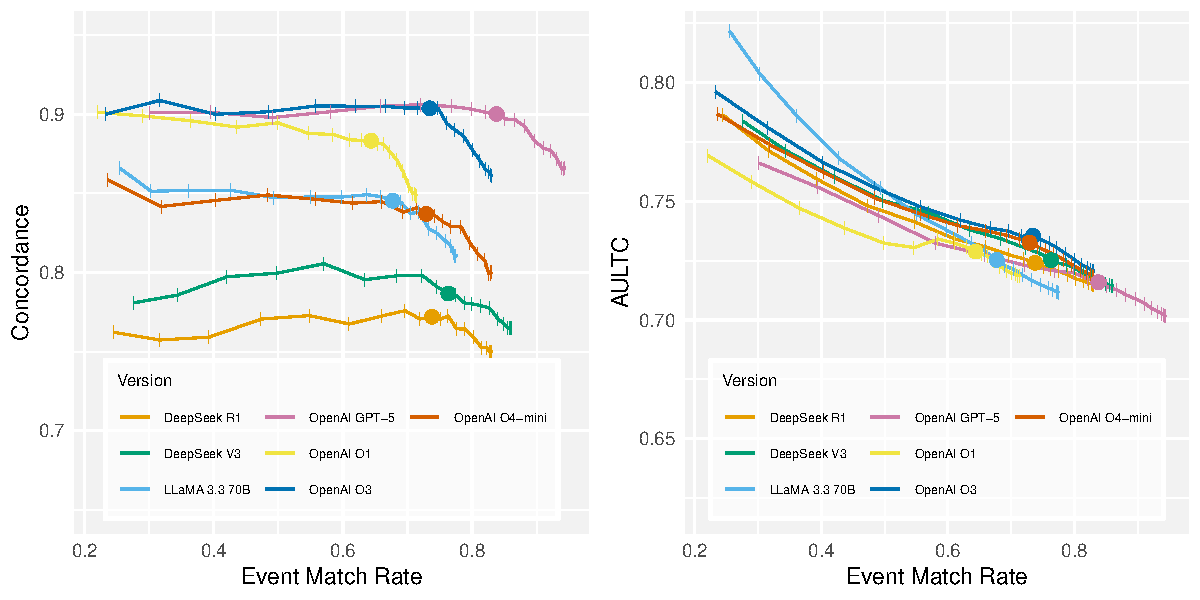
\includegraphics[width=\linewidth]{Plots_tables/event_match_vs_metrics_updated.pdf}
        % \caption{}
    % \end{minipage}
    % \hfill
    \caption{\textbf{A:} Concordance by event match rate. Solid circle ($\bullet$) represents threshold of 0.1, with ticks (|) indicating 0.01 increments of the threshold in [0.01, 0.50]. \textbf{B:} AULTC by event match rate.
    % \textcolor{red}{Remove \texttt{DSR1-quantized} and replace with \texttt{GPT5}. Rerun on 200?}
    }
    \label{fig:threshold_temporal_tradeoff}
    \vspace{-5mm}
\end{figure}

\paragraph{Inter-LLM comparison of temporal annotations}
Finally, We qualitatively compared temporal annotations produced by several LLMs on a representative case report to illustrate characteristic differences in event extraction and timestamping (\textcolor{blue}{Supplementary Material Section~\ref{apd:inter-llm-comparison} Figure~\ref{fig:tts_evaluation}}). While all models recovered the major clinical trajectory and preserved temporal polarity, they varied in
event granularity, paraphrasing, and long-range temporal normalization. These differences complement the aggregate quantitative results and highlight the impact of model behavior on the structure of extracted timelines. \textcolor{blue}{Common model-specific error patterns, such as granularity variation, duplicate events, and differences in temporal normalization, are summarized in the Supplementary Material Table~\label{tab:error_taxonomy}.}


%%%%%%%%%%%%%%%%%%%%%%%%%%%%%%%%%%%%%%%%%

\subsection{Limitations and Future Directions}
\label{sec:limitations-and-future-directions}

Our temporal annotation pipeline has several important limitations. First, it operates on case reports from the PubMed Open Access (PMOA) corpus, which often emphasize rare or atypical presentations and differ from routine clinical notes (e.g., progress notes or discharge summaries in MIMIC-III/IV). This may limit direct generalizability to real-world health system documentation. At the same time, case reports offer rich, temporally structured narratives with explicit clinical rationale, making them a useful testbed for developing and stress-testing textual time series methods. Our LLM-based framework is designed to be reusable and, in ongoing work, is being adapted to corpora such as MIMIC-IV discharge summaries for future dataset releases.

Second, we model events as minimally modified text spans aligned to the source narrative. This design choice preserves interpretability and facilitates direct comparison with the underlying text but relies on embedding-based matching for evaluation and does not normalize event content to standard clinical ontologies such as UMLS. Third, representing time with single relative points simplifies annotation and downstream use but cannot fully capture durations or complex temporal relations (e.g., overlapping intervals or recurrent events).

Fourth, our one-to-one recursive event matching strategy emphasizes temporal consistency at the expense of recall, especially when the same clinical concept is expressed multiple times or in conjunctive form.  Alternative matching formulations (e.g., many-to-many or cluster-based matching) could improve coverage but would require more elaborate evaluation protocols. Finally, the manual reference set comprises 200 cases annotated by a single clinical expert, so we cannot estimate inter-annotator agreement, and all metrics reflect agreement with that expert rather than an adjudicated consensus.

These limitations point to several directions for future work, including ontology-aware event normalization, richer temporal representations (intervals and uncertainty), improved matching algorithms, and extension of the pipeline to diverse EHR-derived note types.

\input{Scientific_data/Supplementary/prompt_ablation}

%%%%%%%%%%%%%%%% Downsteam application : Survival analyses 
%%%%%%%%%%%%%%%%%%%%%%%%%%%%%%%%%%%%%%%%

\section{Downstream Application: Survival Analysis}
\label{sec:downstream-application}

We first evaluated whether the extracted textual time series contain information predictive of time to death by formulating a classical survival analysis task. Many case reports specify whether the patient died and, if so, when (e.g., ``the patient died on hospital day 10''), which enables us to define a time-to-event outcome using the \texttt{death\_info} field. For this task, we evaluate models at predefined cut-off times—specifically at 0 hours (admission), 24 hours (1 day), and 168 hours (1 week)—and use the extracted event history up to each cut-off as input. For each case, the sequence of (event, time) pairs is transformed into a fixed-length embedding using a range of pre-trained language models, including encoder-only transformers (e.g., \texttt{bert-base-uncased}, \texttt{roberta-base}, \texttt{ModernBERT}) and larger decoder-style LLMs (e.g., \texttt{Llama 3.3 70B}, \texttt{DeepSeek-R1} and related distilled variants). We additionally include open-source decoder models with documented training corpora (\texttt{OLMo-2-0325-32B-Instruct}, \texttt{RedPajama-INCITE-7B-Instruct}) and a medically fine-tuned decoder model (\texttt{MediPhi-PubMed}) to examine potential domain-specific benefits and mitigate data-leakage concerns. These embeddings are then used as covariates in standard time-to-event models (DeepSurv and DeepHit) trained to predict survival beyond each cut-off. Model performance is summarized using the time-dependent concordance index to assess alignment between predicted and observed survival times. \textcolor{blue}{Detailed preprocessing, censoring, and hyperparameter tuning procedures are described in the Supplementary Methods Section~\ref{apd:survival-analysis-pipeline}.}

%\input{Scientific_data/Supplementary/survival_table}

%\paragraph{Survival analyses results:}
We report results using \texttt{DeepSeek-R1} annotations only (Table~\ref{tab:survival}). Embeddings derived from larger decoder-style LLMs—particularly \texttt{Llama-3.3-70B-Instruct} and \texttt{DeepSeek-R1-Distill-Llama-70B}—yield the highest time-dependent concordance across cut-offs, followed by their smaller variants and then encoder-only baselines such as \texttt{bert-base-uncased}, \texttt{roberta-base}, and \texttt{ModernBERT}. Open-source decoder models with documented training corpora, including \texttt{OLMo-2-0325-32B-Instruct} and \texttt{RedPajama-INCITE-7B-Instruct}, achieve concordance comparable to mid-sized proprietary LLMs, while the medically fine-tuned \texttt{MediPhi-PubMed} performs similarly to or slightly better than general-domain encoders, suggesting a modest benefit from domain-specific adaptation without relying on private EHR data. Across annotation sources and model families, time-dependent concordance values remain well above 0.7 even at the 1-week horizon, indicating that textual representations of clinical event trajectories carry meaningful signal for time-to-death prediction. These results support the viability of text-to-time modeling on PMOA--TTS and highlight that both representation capacity and training data of the underlying language model substantially influence survival analysis performance.

% \input{Scientific_data/Supplementary/survival_table}

\begin{table*}[t]
\footnotesize
\centering
\begin{adjustbox}{width=\textwidth}
\begin{threeparttable}
\caption{Time-dependent concordance (mean $\pm$ standard deviation across 5 experimental runs) index across embedding models and survival modeling approaches at different time thresholds for DeepSeek annotations.}
\label{tab:survival}
\begin{tabular}{lcccccc}
\toprule
\multirow{2}{*}{\textbf{Embedding Model}} &
\multicolumn{2}{c}{\textbf{Time Threshold = 0h}} &
\multicolumn{2}{c}{\textbf{Time Threshold = 24h}} &
\multicolumn{2}{c}{\textbf{Time Threshold = 168h}} \\
\cmidrule(lr){2-3} \cmidrule(lr){4-5} \cmidrule(lr){6-7}
 & \textbf{DeepHit} & \textbf{DeepSurv} & 
   \textbf{DeepHit} & \textbf{DeepSurv} &
   \textbf{DeepHit} & \textbf{DeepSurv} \\
\midrule

DeepSeek-R1-Distill-Llama-70B     & 0.815 $\pm$ 0.010 & 0.812 $\pm$ 0.013 & 0.815 $\pm$ 0.012 & 0.818 $\pm$ 0.009 & 0.810 $\pm$ 0.012 & 0.812 $\pm$ 0.014 \\
DeepSeek-R1-Distill-Llama-8B      & 0.806 $\pm$ 0.015 & 0.803 $\pm$ 0.011 & 0.809 $\pm$ 0.013 & 0.806 $\pm$ 0.011 & 0.802 $\pm$ 0.010 & 0.809 $\pm$ 0.011 \\
Llama-3.1-8B-Instruct             & 0.815 $\pm$ 0.008 & 0.813 $\pm$ 0.010 & 0.817 $\pm$ 0.010 & 0.811 $\pm$ 0.007 & 0.808 $\pm$ 0.014 & 0.809 $\pm$ 0.011 \\
Llama-3.3-70B-Instruct            & \textbf{0.822 $\pm$ 0.004} & \textbf{0.817 $\pm$ 0.011} & \textbf{0.821 $\pm$ 0.010} & \textbf{0.819 $\pm$ 0.005} & \textbf{0.819 $\pm$ 0.009} & \textbf{0.822 $\pm$ 0.009} \\
ModernBERT-base                   & 0.718 $\pm$ 0.011 & 0.729 $\pm$ 0.008 & 0.733 $\pm$ 0.010 & 0.738 $\pm$ 0.011 & 0.725 $\pm$ 0.013 & 0.729 $\pm$ 0.009 \\
ModernBERT-large                  & 0.653 $\pm$ 0.014 & 0.667 $\pm$ 0.009 & 0.655 $\pm$ 0.015 & 0.665 $\pm$ 0.017 & 0.643 $\pm$ 0.011 & 0.662 $\pm$ 0.003 \\
roberta-base                      & 0.743 $\pm$ 0.013 & 0.746 $\pm$ 0.008 & 0.742 $\pm$ 0.014 & 0.748 $\pm$ 0.006 & 0.744 $\pm$ 0.009 & 0.747 $\pm$ 0.010 \\
deberta-v3-small                  & 0.739 $\pm$ 0.010 & 0.736 $\pm$ 0.010 & 0.730 $\pm$ 0.019 & 0.758 $\pm$ 0.006 & 0.733 $\pm$ 0.012 & 0.751 $\pm$ 0.006 \\
roberta-base                      & 0.757 $\pm$ 0.017 & 0.756 $\pm$ 0.013 & 0.760 $\pm$ 0.012 & 0.758 $\pm$ 0.014 & 0.761 $\pm$ 0.009 & 0.762 $\pm$ 0.011 \\
% \midrule
BioClinical-ModernBERT-base       & 0.696 $\pm$ 0.013 & 0.708 $\pm$ 0.017 & 0.689 $\pm$ 0.010 & 0.717 $\pm$ 0.013 & 0.713 $\pm$ 0.022 & 0.724 $\pm$ 0.018 \\
BioClinical-ModernBERT-large      & 0.637 $\pm$ 0.012 & 0.646 $\pm$ 0.007 & 0.629 $\pm$ 0.012 & 0.647 $\pm$ 0.023 & 0.626 $\pm$ 0.030 & 0.647 $\pm$ 0.022 \\
MediPhi-PubMed                    & 0.780 $\pm$ 0.015 & 0.738 $\pm$ 0.007 & 0.767 $\pm$ 0.016 & 0.781 $\pm$ 0.009 & 0.782 $\pm$ 0.018 & 0.784 $\pm$ 0.022 \\
OLMo-2-0325-32B-Instruct          & 0.800 $\pm$ 0.011 & 0.797 $\pm$ 0.006 & 0.785 $\pm$ 0.015 & 0.790 $\pm$ 0.021 & 0.789 $\pm$ 0.025 & 0.800 $\pm$ 0.027 \\
RedPajama-INCITE-TB-Instruct      & 0.778 $\pm$ 0.014 & 0.742 $\pm$ 0.015 & 0.771 $\pm$ 0.015 & 0.763 $\pm$ 0.008 & 0.791 $\pm$ 0.019 & 0.798 $\pm$ 0.018 \\
\bottomrule

\end{tabular}
\end{threeparttable}
\end{adjustbox}
\end{table*}

%%%%%%%%%%%%%%%%%%%%%%%%%%%%%%%%%%%%%%%%%
%%%%%%%%%%%%%%%% Usage Notes %%%%%%%%%%%%
%%%%%%%%%%%%%%%%%%%%%%%%%%%%%%%%%%%%%%%%

\section{Usage Notes}
\label{sec:usage-notes}

Our full codebase, including preprocessing scripts, prompt templates, and evaluation pipelines,
is available at: \url{https://github.com/jcweiss2/pmoa_tts}. Each subdirectory contains its own README.md with detailed instructions and information. Here is the repository structure
\begin{itemize}
    \item \texttt{make\_tts}: Scripts and notebooks for constructing the PMOA-TTS dataset from case reports.
    \item \texttt{forecasting\_results}: Code for forecasting experiments on the textual time series data.
    \item \texttt{survival\_analyses}: Tools for survival prediction tasks using the extracted timelines.
    \item \texttt{TTS\_evaluation}: Evaluation scripts assessing the quality of the extracted timelines.
\end{itemize}

\noindent Here are step-by-step directions on how to use the dataset

\begin{enumerate}

\item \textbf{Clone the repository:}

{\small
\begin{verbatim}
    git clone https://github.com/jcweiss2/pmoa_tts.git
    cd pmoa_tts
\end{verbatim}
}

\item \textbf{Set up the environment:}

\noindent Ensure you have Python 3.10 or higher installed. It's recommended to use a virtual environment.

{\small
\begin{verbatim}
    conda create -n pmoa_tts python=3.10
    conda activate pmoa_tts
    conda install pandas scikit-learn numpy tensorboard -c conda-forge
    conda install pytorch torchvision torchaudio -c pytorch
    pip install transformers
    pip install argparse
    conda install jupyter -c conda-forge
    pip install sentencepiece
\end{verbatim}
}

\item \textbf{Access the PMOA--TTS dataset.} The dataset is available on Hugging Face. You can download it using the \texttt{datasets} library.

{\small
\begin{verbatim}
    from datasets import load_dataset
    dataset = load_dataset("snoroozi/pmoa-tts")
\end{verbatim}
}

\end{enumerate}

\paragraph{Responsible reuse and cautions}

The release and use of PMOA–TTS raise important considerations. Although LLMs achieve strong performance, they may still generate inaccurate or hallucinated outputs, and any downstream use of these annotations without further validation could introduce bias or error. The extraction of structured diagnoses, demographics, and clinical events from public text—though non-identifiable—could also lead to misinterpretation or reinforce historical biases if not handled carefully. Furthermore, while the dataset is intended for research, there is a risk of misapplication in high-stakes clinical settings without expert oversight. Lastly, the stylistic and structural differences between case reports and real-world EHR notes may limit the generalizability of findings derived from PMOA–TTS. These limitations underscore the importance of using the corpus responsibly, with clear reporting of model limitations and appropriate safeguards when applied in downstream tasks.

%%%%%%%%%%%%%%%%%%%%%%%%%%%%%%%%%%%%%%%%%
%%%%%%%%%%%%%%%%%%%%%%%%%%%%%%%%%%%%%%%%

\section*{Code availability}\label{sec:data_availability}
In line with the philosophy of reproducible research, all codes used in this paper, including those for data preprocessing and technical validation, are accessible at \url{https://github.com/jcweiss2/pmoa_tts}. The usage instructions and parameter settings for all codes can be found at this link.

\bibliography{Scientific_data/references}

\clearpage
\appendix
\input{Scientific_data/supplementary_v2plus}

\end{document}
